\chapter{System Design}\label{cap:sysdes}
Following the requirements and constraints established in the previous chapters, the proposed solution was designed as a modular classroom prototype. Its purpose is not to function as a fully automated assessment platform, but to connect student-side EEG acquisition, local stream transport, teacher-side processing, and post-lesson review into a coherent workflow for observing engagement during teaching activities.



\section{Concept Overview}\label{sect:concov}
At concept level, the system gives the teacher an additional source of information about classroom engagement during technology-supported lessons. It does not replace teacher judgement, evaluate students automatically, or make definitive claims about learning outcomes. Instead, it collects EEG samples from participating students, converts them into an engagement indicator, and presents the result in a form that supports reflection on lesson pacing, topic difficulty, and moments where attention may decrease. The value is treated as an indicator rather than an absolute measurement, since classroom EEG is influenced by movement, electrode contact, individual variation, and environmental noise; this cautious interpretation follows previous classroom EEG studies, where engagement monitoring is treated as supportive information rather than as a direct measure of learning \cite{Poulsen2017,Apicella2022,Xu2018,BustosLopez2022}.


In the intended classroom scenario, each student uses one Unicorn EEG headset connected to one Raspberry Pi acquisition node, and this station is repeated for \(N\) students, with every station publishing its stream to the same local network. The student-side node is kept deliberately simple: its role is limited to acquisition and transmission, without any pedagogical decision-making. On the teacher workstation, the application receives the available streams, identifies them by student or device label, computes the engagement value, and displays the information through a Streamlit interface. Keeping interpretation, visualization, lesson management, and reporting on the workstation creates a complete path from physiological acquisition to classroom-facing feedback, and means that changes to the metric or to the interface do not require the acquisition nodes to be redesigned.


The interface is teacher-centered: rather than ranking students or building permanent profiles, it focuses on lesson activity and class-level reflection, so the teacher can relate changes in engagement to instructional decisions without reducing students to a single numerical score. Because a live signal monitor alone would not be sufficient for this, the prototype also includes the surrounding teaching workflow, where materials can be uploaded, previewed, presented, and later reviewed through reports. EEG-derived engagement becomes more meaningful this way: a decrease during a particular slide is more useful when the teacher can relate it to the topic or activity taking place at that moment.

\section{Architecture and Data Flow}\label{sect:archndf}
Architecturally, the prototype is organized around four main parts: acquisition nodes, stream transport, teacher-side processing, and local storage. Acquisition nodes interact with the EEG headsets, the transport layer makes streams discoverable on the local network, the teacher application receives and interprets the data, and local storage preserves lesson materials, generated previews, configuration data, and report information. This separation gives the system a clear structure and allows each part to be tested with limited dependence on the others.


Data flow begins at the student-side unit. The Unicorn headset provides the EEG signal, and the paired Raspberry Pi acquisition node forwards that signal as an LSL stream. Stream metadata identifies the device and student label, which allows the teacher application to distinguish between several participants. By using distributed acquisition nodes, the teacher workstation does not need to manage direct headset connections, which would become increasingly difficult as more students are added.


When a stream becomes available on the local network, the teacher application discovers it and opens a receiving inlet. Incoming samples are stored in a stream state containing the current signal value, packet count, connection freshness, stream metadata, and in-session history. The attention-processing component receives the selected EEG values and produces an engagement estimate, while the user interface reads the organized state and presents it through cards, detail views, charts, and reports.


This stream state functions as the main internal representation on the teacher side. Interface pages do not work directly with network connections; they work with structured information about each detected participant stream. Such an arrangement makes the visual layer more stable, because streams can appear, become quiet, or disappear without forcing the whole interface to change its structure.


Classroom conditions also motivated a tolerant startup model. A lesson can be prepared even when no headset is currently streaming. A Raspberry Pi can be deployed or validated from the administration page before teaching begins. New streams may also appear after the teacher application has already started, because discovery is performed dynamically. This flexibility is useful in practical teaching environments, where setup time is limited and devices may not all become available at the same moment.


Two information paths meet inside the teacher application. One path is physiological: headset, acquisition node, LSL stream, collector, attention metric, visualization. The other is instructional: uploaded material, local preview, presentation, report. Bringing these paths together prevents engagement information from being shown in isolation and makes it possible to relate the signal to the activity taking place during the lesson.

Figure~\ref{fig:hardware_deployment} presents the hardware side of this separation. The left part of the diagram represents one student station: the student wears the Unicorn headset, the Raspberry Pi reads the device through the vendor library, and the Pi streamer publishes the resulting signal. This station is repeated for each participant, while the teacher workstation remains the single point where the streams are observed and interpreted.

\begin{figure}[h]
\centering
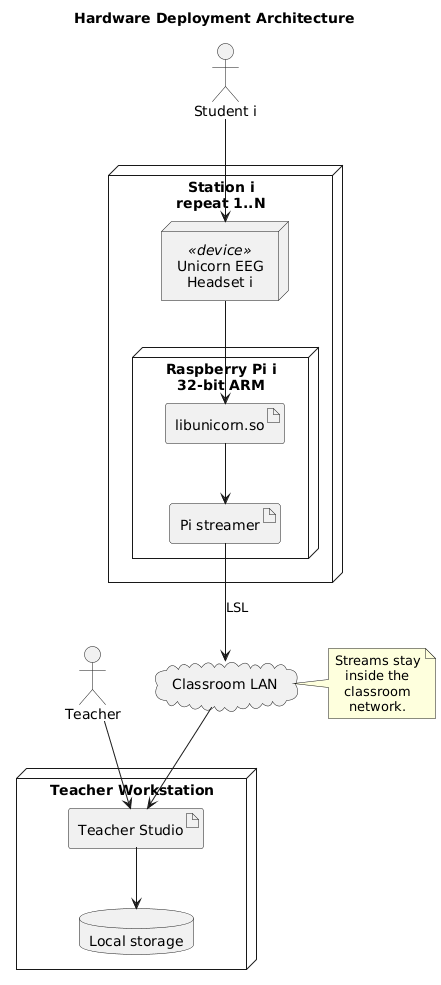
\includegraphics[width=0.82\textwidth,height=0.68\textheight,keepaspectratio]{En/UML_hardware_diagram.png}
\caption{Hardware deployment architecture for the classroom prototype. Each student station contains one Unicorn headset and one Raspberry Pi acquisition node, while the teacher workstation receives the resulting LSL streams over the classroom network.}
\label{fig:hardware_deployment}
\end{figure}

The classroom workflow is intentionally sequential from the teacher's perspective: setup and validation happen before the lesson, while monitoring, presentation, and report review happen during and after teaching. Figure~\ref{fig:application_flow} summarizes this operational flow.


\begin{figure}[h]
\centering
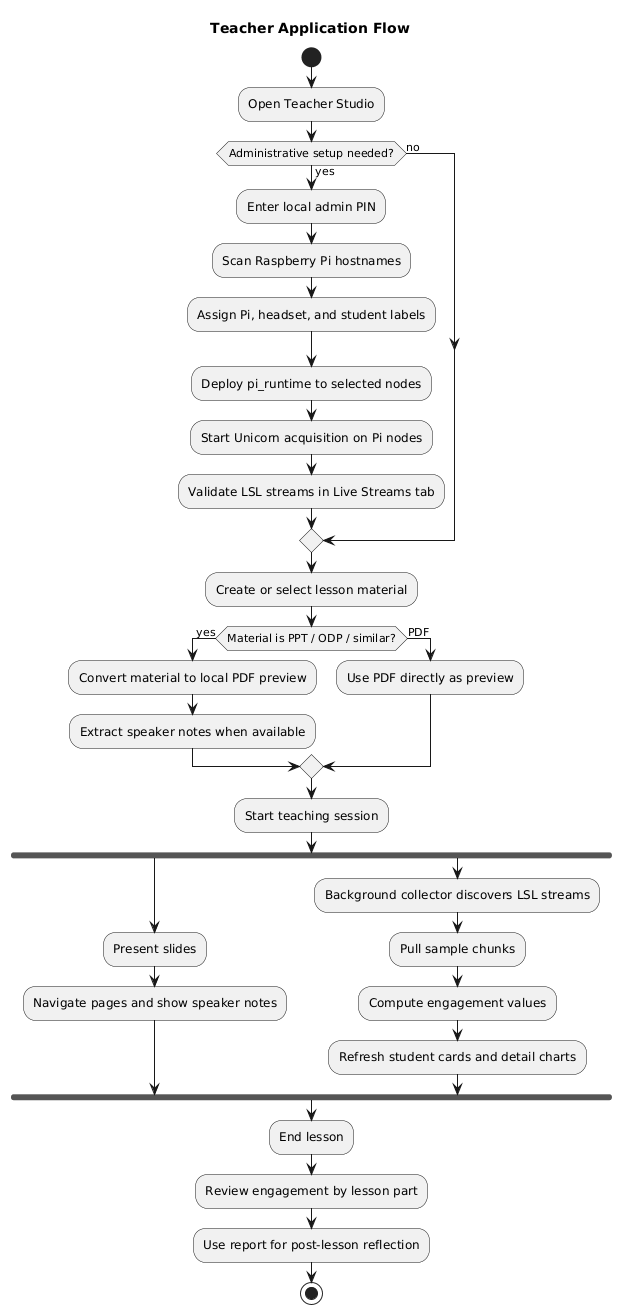
\includegraphics[width=0.82\textwidth,height=0.68\textheight,keepaspectratio]{En/UML_app_flow.png}
\caption{Application workflow from device preparation and stream validation to lesson presentation and post-lesson review.}
\label{fig:application_flow}
\end{figure}

The activity diagram is useful because it shows that the prototype is not only a signal viewer. It starts with administration tasks such as device preparation and stream validation, then moves into lesson selection and presentation, and only after the lesson does it enter the reporting stage. This matches the way the application is intended to be used in a real teaching session.


\section{Hardware Setup}\label{sect:hwset}
For the hardware layer, the prototype uses a distributed acquisition model. Instead of connecting all EEG devices directly to the teacher workstation, each student-side headset is paired with a nearby Raspberry Pi node, forming one acquisition station for that student. You can see an example of such a station in Figure~\ref{fig:hardware_setup} A classroom deployment can contain \(N\) such stations, but a single student does not share or control multiple stations. The Pi handles device access and stream publication, while the teacher workstation receives standardized streams over the local network. In a classroom setting, this reduces the amount of direct hardware management required on the teacher computer.

As signal source, the system uses the Unicorn EEG headset. The Raspberry Pi acts as a compact acquisition computer that runs the device interface and publishes the resulting stream. Each acquisition point can therefore be treated as an independent unit. If another participant is added, another acquisition node can be prepared without changing the teacher-side architecture.

\begin{figure}[h]
\centering
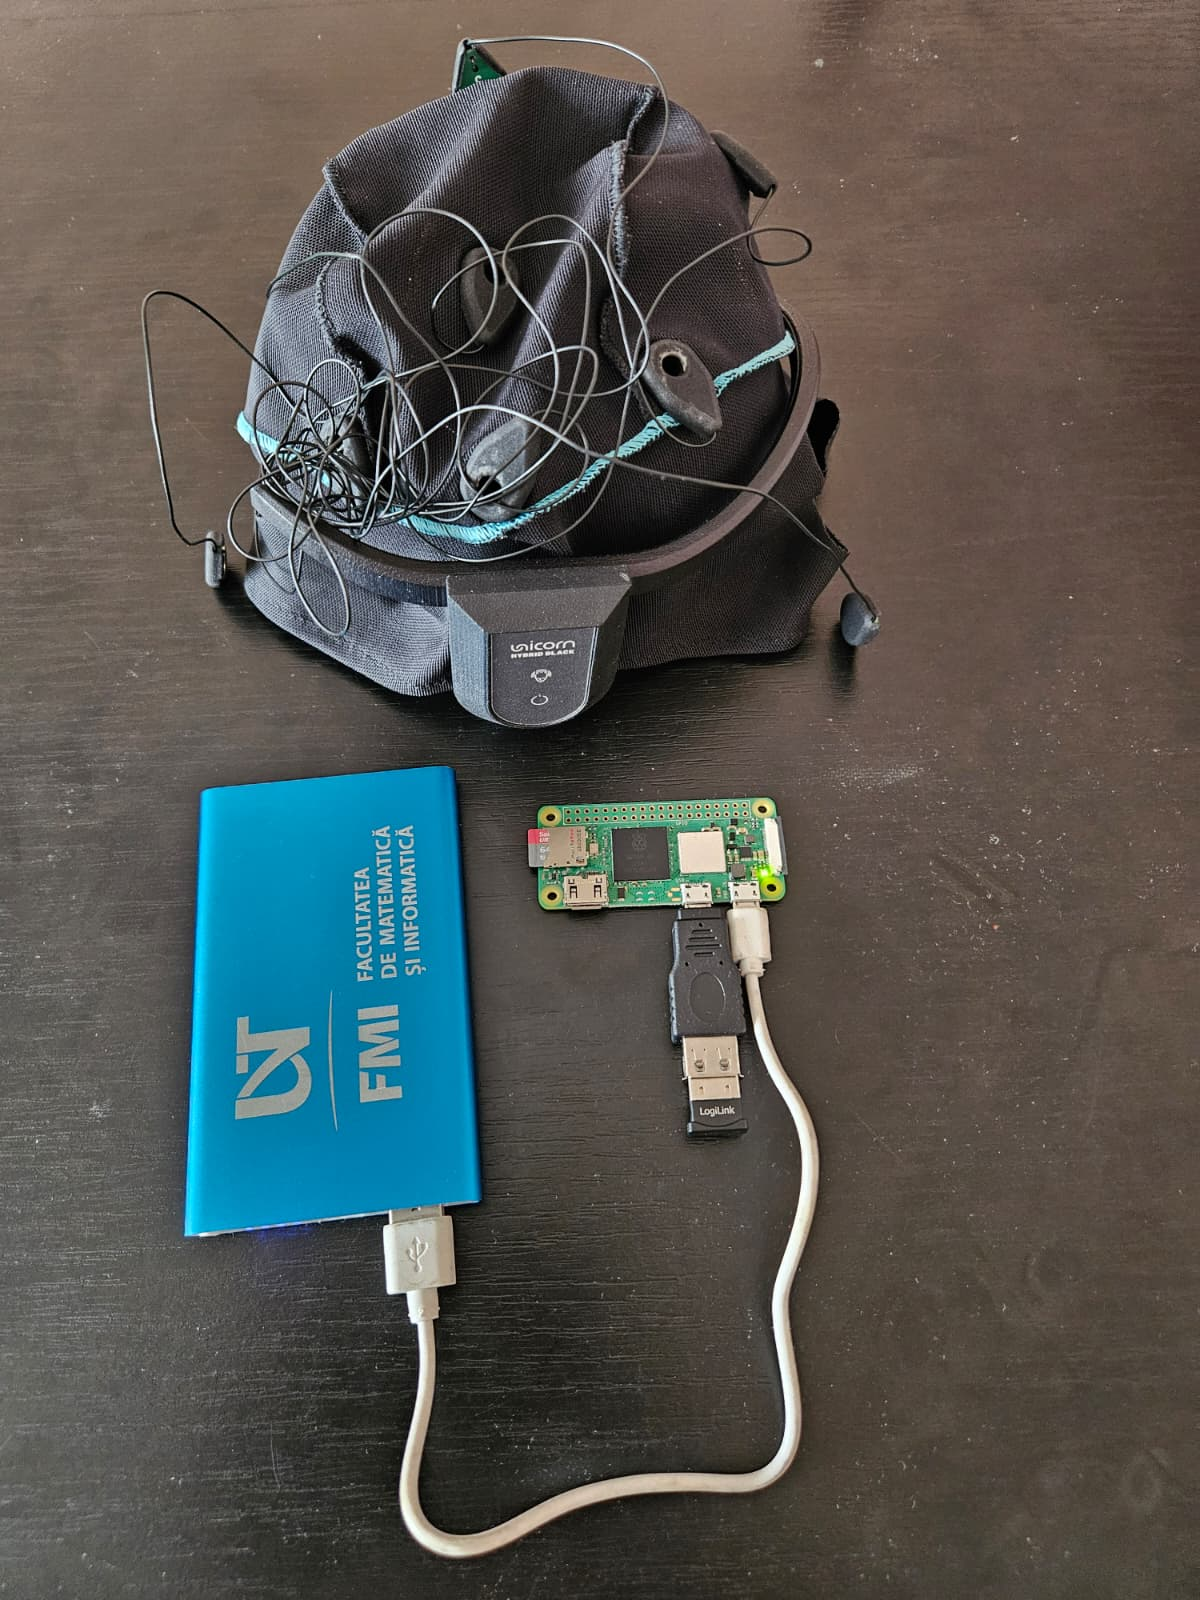
\includegraphics[width=0.92\textwidth]{En/1. Student Station.jpeg}
\caption{Student acquisition station setup showing only the power bank, Raspberry Pi, and Unicorn EEG headset.}
\label{fig:hardware_setup}
\end{figure}

This organization also gives more freedom in classroom placement. The acquisition node can remain close to the student-side device, while the teacher workstation can stay where the lesson is controlled. A design based on direct connections between all headsets and one central machine would be less convenient and more fragile in a normal classroom arrangement.


A practical constraint comes from the vendor library used by the acquisition runtime. The included Unicorn Pi Zero W library targets a 32-bit ARM environment, so the Raspberry Pi setup must be compatible with that requirement. Before any network streaming or signal handling can take place, the acquisition node must be able to load the native library and communicate with the headset.


On the teacher side, the workstation is a standard Windows computer running the Python environment and the Streamlit application. It receives LSL streams, manages lesson materials, runs the engagement processing, and displays the interface. Since no EEG device has to be connected directly to this computer, the setup remains closer to a normal classroom laptop than to a laboratory acquisition station.


Real-time communication is intended to remain local. The core classroom workflow does not depend on cloud services, which makes the prototype usable even when internet access is limited or unreliable. Internet connectivity may still be needed for installation or dependency setup, but teaching, streaming, processing, and review are designed to operate within the local environment.

\section{Software Components}\label{sect:swcomp}
From a software perspective, the system is divided into an acquisition runtime and a teacher application. The runtime executes on the Raspberry Pi and exposes headset data through LSL. The teacher application runs on the workstation and contains the collector, processing module, user interface, lesson services, report view, and administration tools. This division keeps the embedded side focused while placing the more complex interaction logic on the machine used by the teacher.


Figure~\ref{fig:software_architecture} gives the general software organization. The Raspberry Pi side is limited to the bridge between the Unicorn device and the LSL outlet. The LSL layer carries both samples and metadata. On the workstation, the teacher application is split into pages, live acquisition logic, lesson/report services, administration services, and reusable UI components.

\begin{figure}[h]
\centering
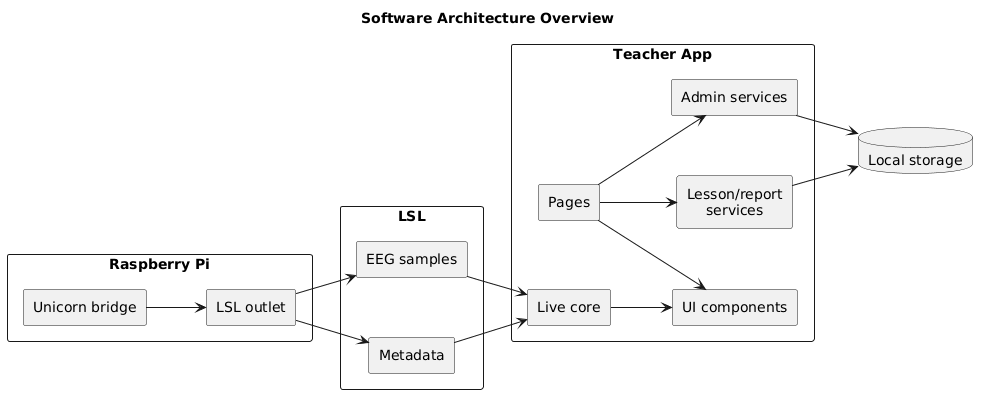
\includegraphics[width=0.92\textwidth]{En/UML_software_diagram.png}
\caption{General software architecture showing the Raspberry Pi runtime, LSL transport, teacher application modules, and local storage.}
\label{fig:software_architecture}
\end{figure}
Within the acquisition runtime, the main responsibility is bridging the native device library and the LSL network. It opens the headset, selects the configured stream mode, attaches metadata, and publishes the signal. The component does not need to know how lessons are presented or how reports are generated, which keeps it reusable and easier to debug.


The acquisition runtime is shown in more detail in Figure~\ref{fig:software_pi_runtime}. The launcher starts the C API streamer, the streamer accesses the vendor library through Python bindings, and the outlet publishes the signal to the classroom network. Keeping this chain short makes failures easier to isolate: device access problems remain on the Pi side, while visualization and interpretation remain on the teacher workstation.

\begin{figure}[h]
\centering
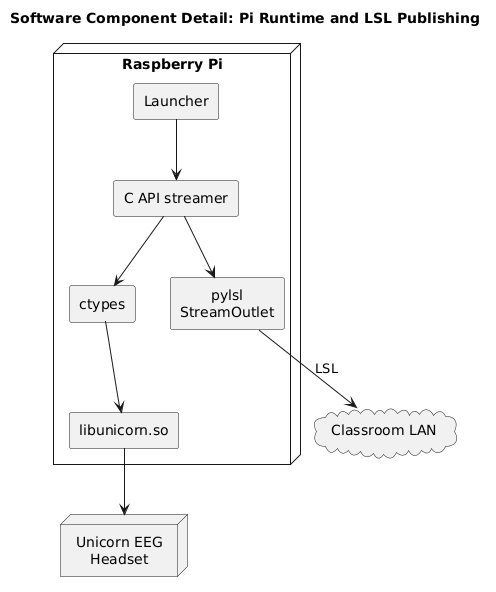
\includegraphics[width=0.7\textwidth]{En/UML_software_pi_runtime.png}
\caption{Pi-side software components used to access the Unicorn device and publish EEG samples through an LSL outlet.}
\label{fig:software_pi_runtime}
\end{figure}

On the workstation, the teacher application is organized into pages and supporting services. Pages define the visible workflow: dashboard, lesson creation, teaching, reports, and administration. Services handle operations such as saving uploaded materials, preparing previews, extracting speaker notes, collecting LSL streams, and deploying acquisition nodes. This prevents the interface from becoming a single block of mixed presentation and system logic.


Signal interpretation is kept independent from the interface. The attention-processing component receives numerical EEG samples and returns an engagement value. Keeping this logic separate makes the metric easier to explain and isolates the signal-processing assumptions from the rest of the application. In future work, a different metric could be introduced without redesigning the lesson pages or the administration workflow.


Figure~\ref{fig:software_live_monitoring} shows the live monitoring path inside the teacher application. The collector service provides access to a background collector, the collector reads LSL samples and metadata, and the attention metric produces engagement updates. The UI does not communicate directly with LSL; it renders snapshots of the stream state, which keeps the interface responsive even when streams appear, become quiet, or disappear.

\begin{figure}[h]
\centering
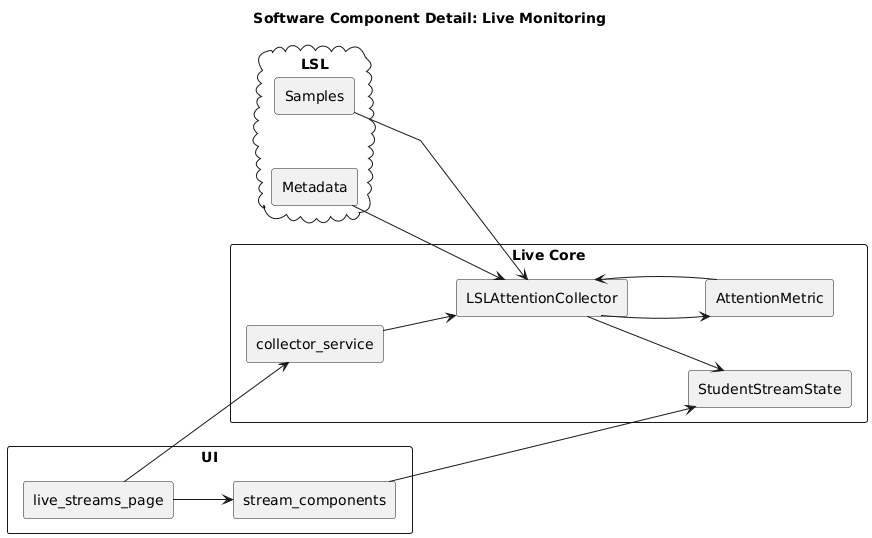
\includegraphics[width=0.9\textwidth]{En/UML_software_live_monitor.png}
\caption{Live monitoring components responsible for receiving LSL streams, maintaining stream state, computing engagement values, and rendering the stream inspection interface.}
\label{fig:software_live_monitoring}
\end{figure}

Lesson and report features complete the teacher workflow. Materials are stored locally and can be presented from inside the same application, while reports summarize engagement by lesson part for later review. Together, these components turn the prototype into a coherent teaching tool rather than a collection of unrelated utilities.


Figure~\ref{fig:software_lesson_reporting} separates the lesson workflow from the live signal workflow. The lesson store manages saved material and metadata, conversion prepares PDF previews when needed, and speaker-note extraction supports presenter view. The reporting component uses lesson segmentation to relate engagement values to meaningful parts of the lesson instead of showing only a raw time series.

\begin{figure}[h]
\centering
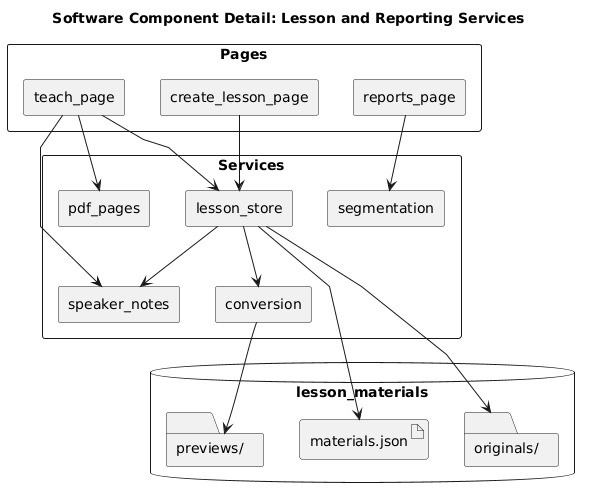
\includegraphics[width=0.88\textwidth]{En/UML_software_lesson_reporting.png}
\caption{Lesson and reporting components used for material upload, preview generation, speaker-note extraction, slide rendering, and post-lesson summaries.}
\label{fig:software_lesson_reporting}
\end{figure}

Administration is included because multi-user acquisition requires preparation before the lesson begins. Devices must be discovered, assigned, deployed, and validated. Keeping these operations in a dedicated area protects the normal teaching pages from unnecessary technical detail while still making setup tasks available when they are needed.

The administration components in Figure~\ref{fig:software_admin_deployment} support this preparation stage. The inventory tab stores Raspberry Pi and headset assignments, the deployment tab uses the PowerShell deployment script to copy and prepare the Pi runtime, and the live streams tab validates that published LSL streams can be discovered by the teacher workstation.

\begin{figure}[h]
\centering
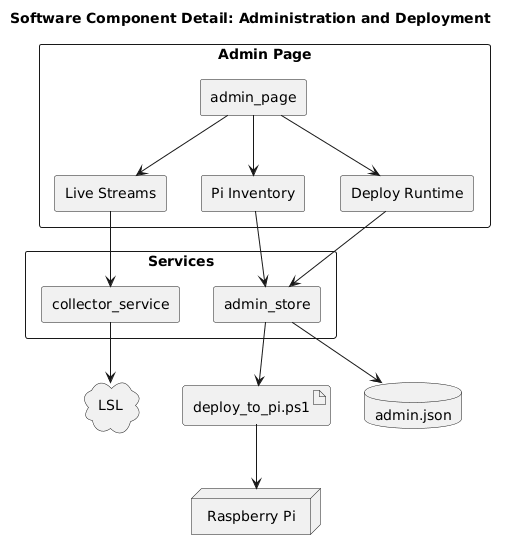
\includegraphics[width=0.8\textwidth]{En/UML_software_admin.png}
\caption{Administration and deployment components used to manage Raspberry Pi inventory, runtime deployment, configuration storage, and stream validation.}
\label{fig:software_admin_deployment}
\end{figure}

\subsection{Lab Streaming Layer Integration}\label{ssect:lsl}
LSL provides the communication boundary between acquisition and interpretation. Each Raspberry Pi publishes a stream, and the teacher workstation discovers and receives available streams on the local network. This avoids custom networking logic and supports a flexible startup order, since acquisition nodes and the teacher interface do not have to be launched in a strict sequence. The choice is also aligned with the intended use of LSL as a framework for timestamped, synchronized data streaming across local networked systems \cite{Kothe2025}.


Metadata attached to the streams is essential for usability. Student labels, device names, channel information, and stream names allow the teacher application to present multiple streams in a readable way. Without this context, the interface would receive numerical samples but would not have enough information to associate them meaningfully with classroom participants.


A further distinction is made between signal timing and interface freshness. LSL timing preserves the meaning of incoming data, while local receipt time helps the interface decide whether a stream appears live, quiet, or stale. In a classroom dashboard, showing whether values are still being updated is almost as important as showing the values themselves.

\subsection{Python Visualization Module}\label{ssect:pyvizmod}
Streamlit was selected for the visualization module because the prototype needs to combine Python-based processing with a usable teacher interface. Its structure follows the teacher's workflow rather than the internal implementation modules. The dashboard gives quick access to the main tasks, while the lesson, teaching, report, and administration pages separate the different moments of use.


The dashboard in Figure~\ref{fig:teacher_dashboard} is the teacher's entry point. It avoids exposing low-level streaming details immediately and instead presents the four main actions: preparing material, teaching, reviewing reports, and entering the administration area. This keeps routine classroom use separate from technical setup tasks.

\begin{figure}[h]
\centering

\includegraphics[width=0.95\textwidth]{\detokenize{En/2. Teacher Dashboard.png}}
\caption{Teacher Studio dashboard with quick access to lesson creation, teaching, reporting, and administration.}
\label{fig:teacher_dashboard}
\end{figure}
Live stream information is shown at two levels of detail. Student cards provide a compact view of engagement and stream status, which is suitable for quick inspection during a lesson. A detailed view exposes raw samples and stream metadata, making it more useful during setup or troubleshooting. This balance is important because normal teaching requires a simple display, while validation sometimes requires deeper technical information.


Figure~\ref{fig:live_stream_cards} illustrates the compact level. Each card combines the student label, engagement value, device identifier, LSL stream name, and freshness status. The stale card is important because it shows how the interface communicates a missing or inactive data source without removing the student from the display.

\begin{figure}[h]
\centering

\includegraphics[width=0.95\textwidth]{\detokenize{En/3a. 4 Student cards with 1 stale.png}}
\caption{Live stream cards showing four configured student streams, including one stale stream where data is no longer being received.}
\label{fig:live_stream_cards}
\end{figure}

\begin{figure}[h]
\centering

\includegraphics[width=0.9\textwidth]{\detokenize{En/3b. Student-01 engagement and metrics.png}}
\caption{Selected-student detail view showing engagement value, stream status, packet count, sample rate, and connection freshness.}
\label{fig:selected_student_metrics}
\end{figure}
Figure~\ref{fig:selected_student_metrics} shows the detailed level for one stream. This view is more technical and is meant for validation or troubleshooting: it exposes packet count, sample rate, last-seen age, status, and the latest engagement value for the selected student.
By connecting lesson activity and engagement monitoring, the interface supports the practical goal of the project. Materials can be prepared, previewed, presented, and later reviewed through reports. Neurofeedback is therefore placed inside the teaching process, rather than being presented as a separate technical instrument that distracts from the lesson.


Unnecessary signal-processing terminology is avoided in the normal teaching flow. Technical details remain available in stream inspection and administration views, but the main workflow is expressed through familiar actions such as creating a lesson, presenting material, and reviewing a report. This makes the system easier to approach in an educational context.

\section{Data Transmission Protocols}\label{sect:commnsync}
Different communication methods are used for live data and management tasks. Real-time EEG samples are transmitted through LSL because they require discovery and timestamped streaming \cite{Kothe2025}. Deployment and maintenance use SSH and SCP, which are more appropriate for remote command execution and file transfer than for continuous signal transmission.


Information that must persist between sessions is stored locally on the teacher workstation. This includes lesson materials, generated previews, configuration files, device inventory, and deployment logs. A local-first design keeps the classroom workflow independent of cloud services and makes the prototype easier to run in a controlled school environment.


Access to administration functions is separated from the normal teaching pages and protected by a local PIN hash. This should not be interpreted as a complete security model for sensitive data, but it provides a basic boundary between everyday teaching actions and technical operations such as deployment or device inventory changes. A production version would require stronger privacy and access-control mechanisms.

\clearpage
